\chapter{集合}
\label{chap:collection}

java容器类可以划分为两个不同的概念

\textbf{Collection} 

一个独立元素的序列。

\begin{itemize}
    \item   List必须按照插入的顺序保存元素
    \item   Set不能有重复元素
    \item   Queue按照队列规则来确定对象产生的顺序
\end{itemize}

ArrayList、LinkedList、ArrayDeque、Vector、Stack

EnumSet、SortedSet、HashSet、TreeSet、LinkedHashSet


\textbf{Map}

一组成对的“键值对”对象,允许你使用键来查找值。

HashMap、TreeMap、LinkedHashMap、WeakHashMap、EnumMap、IdentityHashMap

\begin{figure}[H]
    \centering
    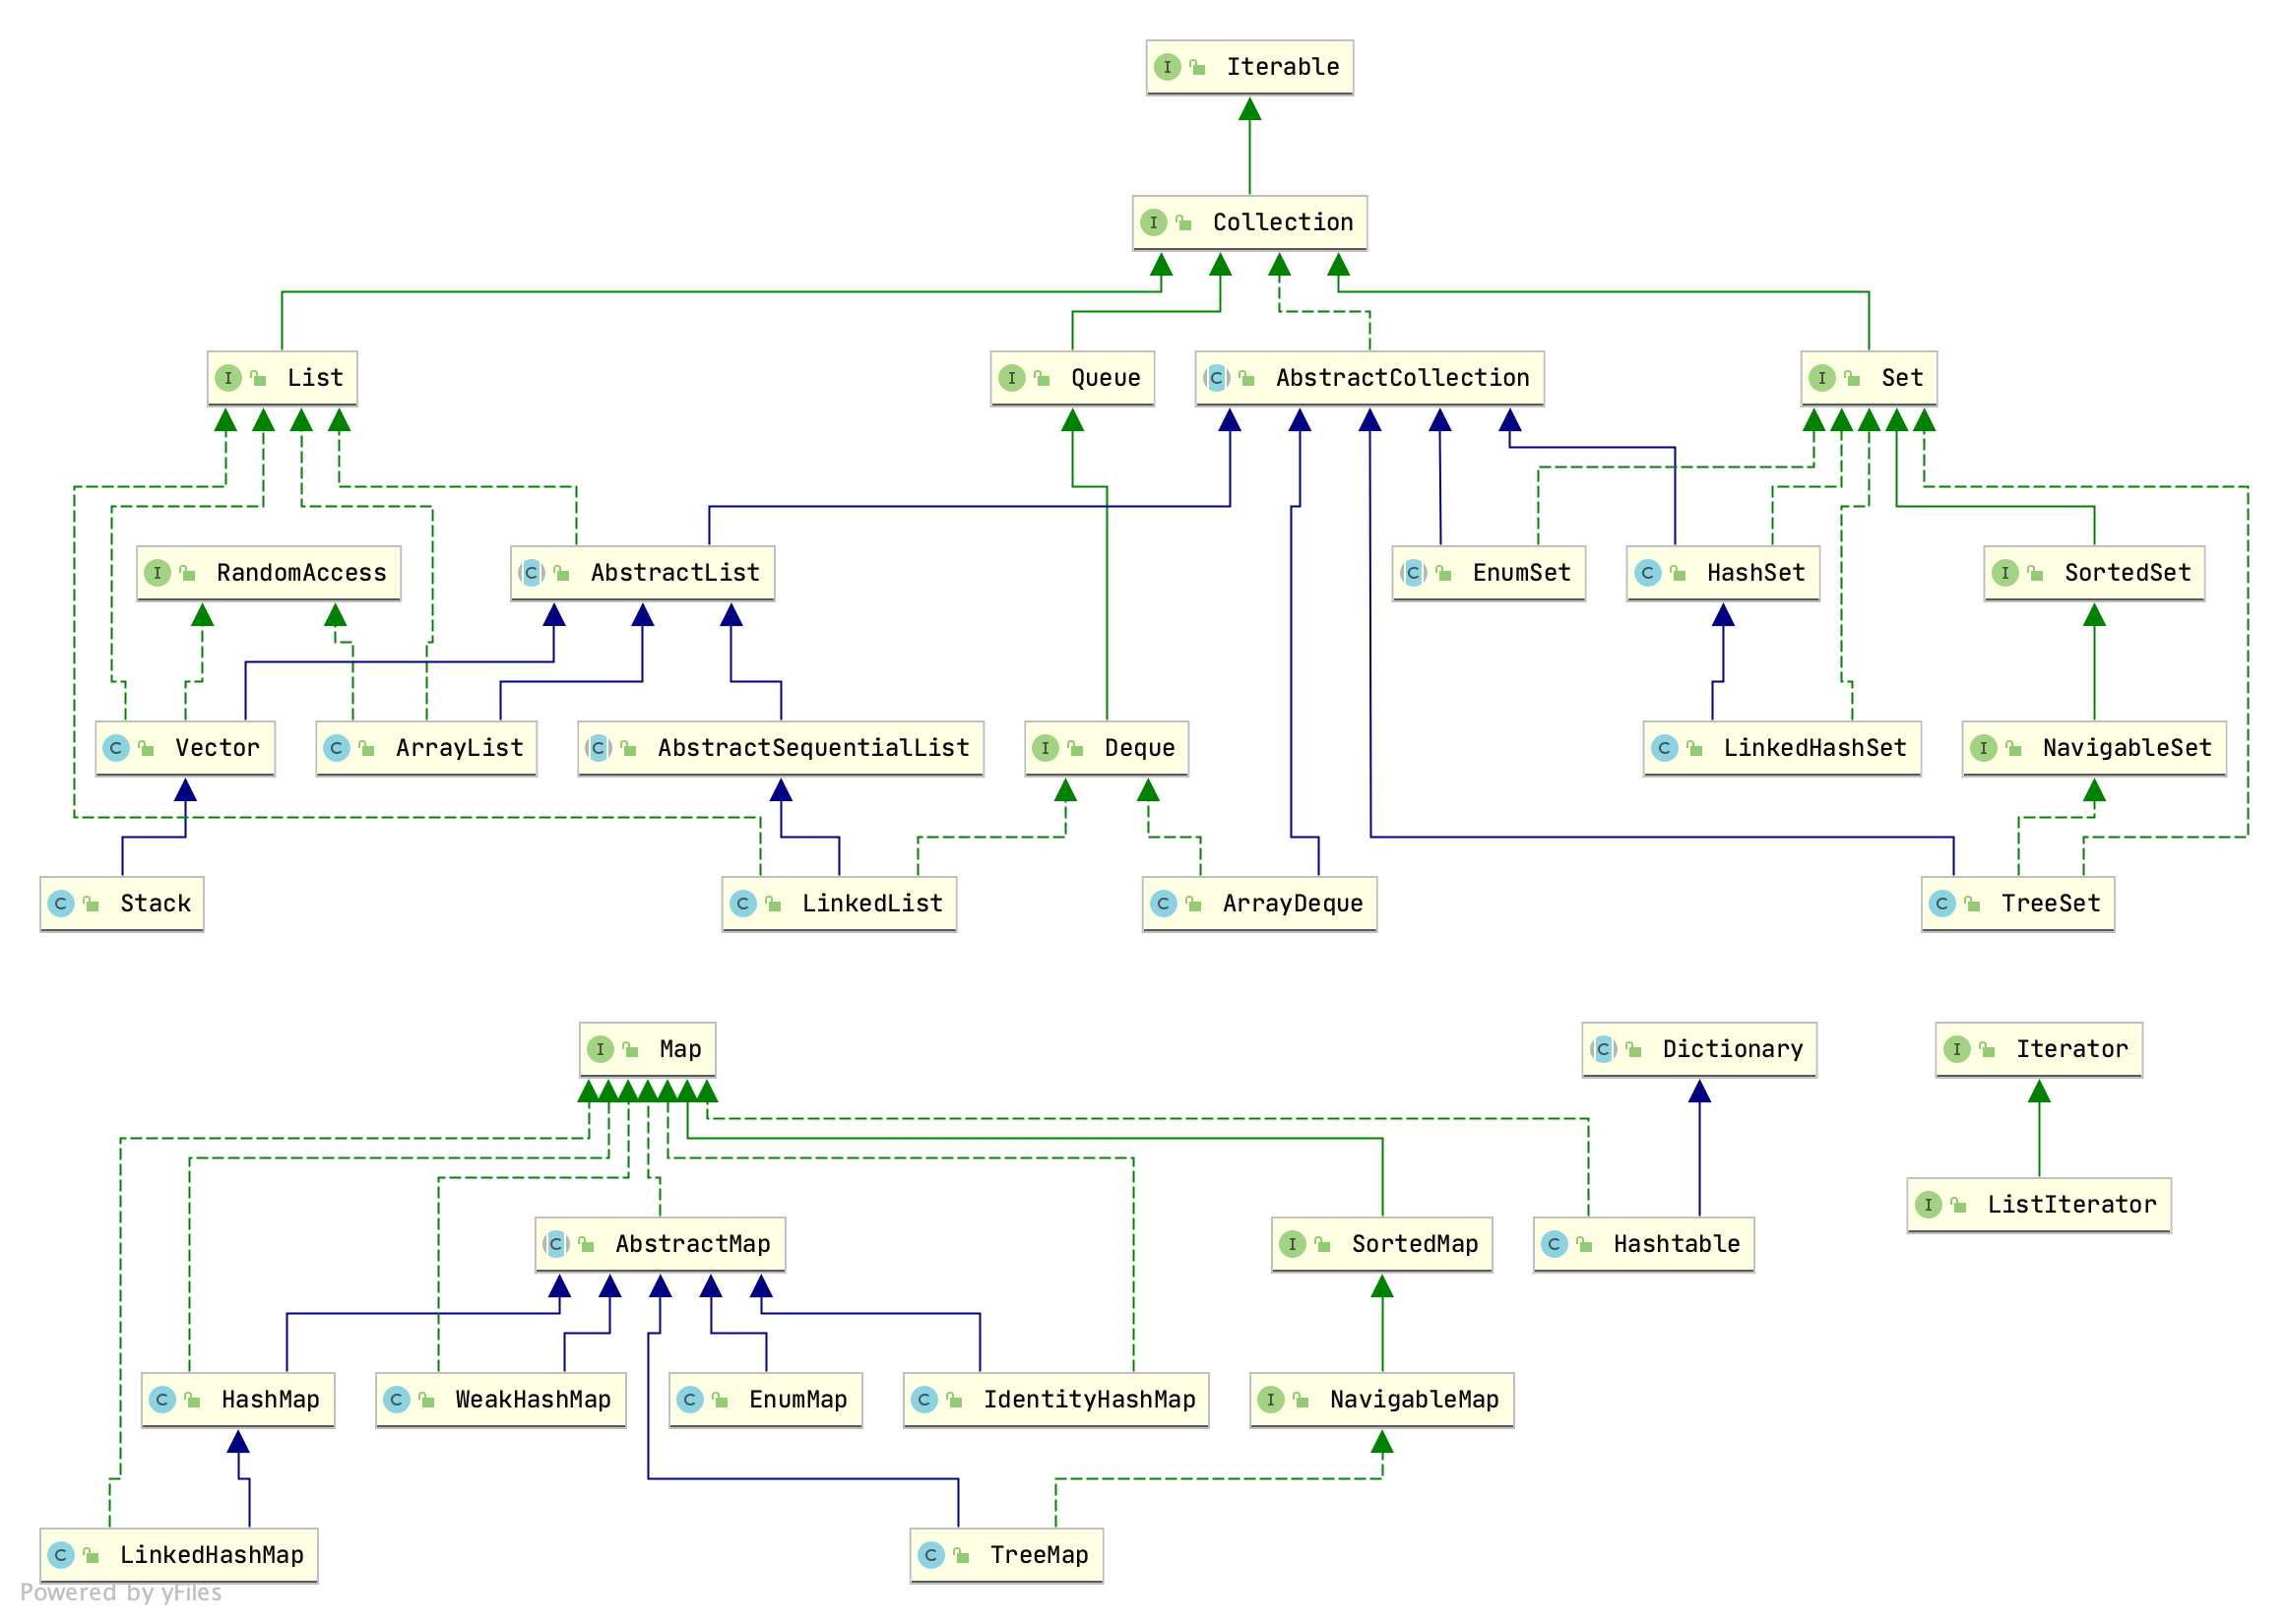
\includegraphics[width=1\textwidth]{collection/collection_impl_class.png}
\end{figure}


\textbf{ArrayList}






Arrays.asList() 产生的List底层为数组,因此不能调整尺寸。







